\documentclass{beamer}
%
% Choose how your presentation looks.
%
% For more themes, color themes and font themes, see:
% http://deic.uab.es/~iblanes/beamer_gallery/index_by_theme.html
%
\mode<presentation>
{
  \usetheme{default}      % or try Darmstadt, Madrid, Warsaw, ...
  \usecolortheme{default} % or try albatross, beaver, crane, ...
  \usefonttheme{default}  % or try serif, structurebold, ...
  \setbeamertemplate{navigation symbols}{}
  \setbeamertemplate{caption}[numbered]
} 

\usepackage[english]{babel}
\usepackage[utf8x]{inputenc}
\usepackage{hyperref}


\title[Sandhi]{Sandhi}
\author{Manoj Gudi}
\institute{R.A. FOSSEE | NME-ICT | IIT Bombay}
\date{7th March 2014}

\begin{document}

\begin{frame}
  \titlepage
\end{frame}

% Uncomment these lines for an automatically generated outline.
%\begin{frame}{Outline}
%  \tableofcontents
%\end{frame}

\section{Introduction}

\begin{frame}{Pre-Sandhi}

\begin{itemize}
  \item LabVIEW: A proprietary visual programming software by NI
  \item Vendor lockdown 
  \item Buy NI DAC cards .. Buy LabVIEW  = \textbf{ \textit{Evil Maxx}}
  \item Little care for support on Free Operating Systems: GNU/Linux.
  \item Main target: Virtual Labs, IIT Bombay.
\end{itemize}

\vskip 1cm

\end{frame}


\section{Main Content}

\vskip 1cm
\begin{frame}{}
\subsection{section}
\begin{figure} [ht!]
	\centering
	
\includegraphics[width=70mm]{meme1.jpg}
\end{figure}
\end{frame}


\section{Main Content}

\begin{frame}{Objectives}

\begin{figure} [ht!]
	\centering
	
\includegraphics[width=60mm]{meme2.jpg}
\end{figure}

\begin{itemize}
  \item Free and Open source
  \item Easy to use | Clean interface | Drag \& Drop 
  \item Should run on GNU/Linux smoothly
  \item Able to carry out control system experiments
  \item Framework should support \textbf{feedbacks}
\end{itemize}

\vskip 1cm

\end{frame}



\section{Main Content}

\begin{frame}{Architecture}

\begin{figure} [ht!]
	\centering
	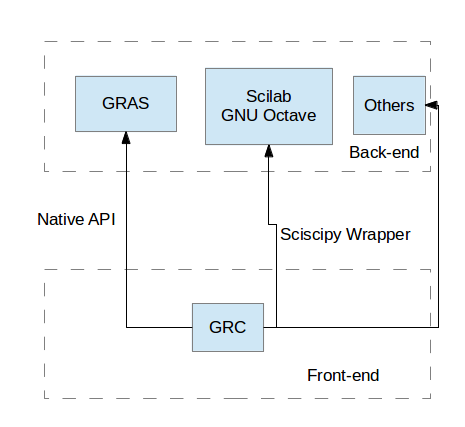
\includegraphics[width=80mm]{image.png}
\end{figure}
\vskip 1cm
\end{frame}


\begin{frame}{Features}

\begin{itemize}
  \item Light-weight \textasciitilde 20mb without depdendencies
  \item Good Hardware driver support
  \item Language support for Development: Scilab, GNU/Octave, Python, C++
  \item Developed for Control system application
  \item But can be easily extended for
  \begin{itemize}
  	\item Image Processing
	\item Neural Networks
	\item And any other areas which can be represented as data-flowgraph
  \end{itemize}
\end{itemize}

\vskip 1cm

\end{frame}


\begin{frame}{References/Links}

\begin{itemize}
  \item Source code \url{https://github.com/gnu-sandhi/sandhi.git}
  \item Documentation \url{https://github.com/gnu-sandhi/docs.git}
  \item Problems using it? Found a bug?
  \begin{itemize}
 	\item Are you sure its a bug and \textbf{not} \textit{a feature}?
	\item Raise a issue on our github
	\item Mailing List: \textit{gnu\_lc@googlegroups.com}
  \end{itemize}
\end{itemize}

\vskip 1cm

\end{frame}

\end{document}
